



\documentclass[
	% -- opções da classe memoir --
	12pt,				% tamanho da fonte
	openright,			% capítulos começam em pág ímpar (insere página vazia caso preciso)
	oneside,			% para impressão em recto e verso. Oposto a oneside
	a4paper,			% tamanho do papel. 
	% -- opções da classe abntex2 --
	%chapter=TITLE,		% títulos de capítulos convertidos em letras maiúsculas
	%section=TITLE,		% títulos de seções convertidos em letras maiúsculas
	%subsection=TITLE,	% títulos de subseções convertidos em letras maiúsculas
	%subsubsection=TITLE,% títulos de subsubseções convertidos em letras maiúsculas
	% -- opções do pacote babel --
	english,			% idioma adicional para hifenização
	french,				% idioma adicional para hifenização
	spanish,			% idioma adicional para hifenização
	brazil				% o último idioma é o principal do documento
	]{abntex2}




% Pacotes básicos 
\usepackage{lmodern}			% Usa a fonte Latin Modern			
\usepackage[T1]{fontenc}		% Selecao de codigos de fonte.
\usepackage[utf8]{inputenc}		% Codificacao do documento (conversão automática dos acentos)
\usepackage{indentfirst}		% Indenta o primeiro parágrafo de cada seção.
\usepackage{color}				% Controle das cores
\usepackage{graphicx}			% Inclusão de gráficos
\usepackage{microtype} 			% para melhorias de justificação
\usepackage{amsmath}			% lib para equacoes
\usepackage{svg}
%\usepackage{float}
\usepackage[T1]{fontenc}
\usepackage{listings}
\usepackage{tikz}
\usepackage{caption}
\usetikzlibrary{shapes.geometric, arrows}

\tikzstyle{startstop} = [rectangle, rounded corners, 
minimum width=3cm, 
minimum height=1cm,
text centered, 
draw=black, 
fill=red!30]

\tikzstyle{io} = [trapezium, 
trapezium stretches=true, % A later addition
trapezium left angle=70, 
trapezium right angle=110, 
minimum width=3cm, 
minimum height=1cm, text centered, 
draw=black, fill=blue!30]


\tikzstyle{process} = [rectangle, 
minimum width=3cm, 
minimum height=1cm, 
text centered, 
text width=3cm, 
draw=black, 
fill=orange!30]

\tikzstyle{decision} = [diamond, 
minimum width=3cm, 
minimum height=1cm, 
text centered, 
draw=black, 
fill=green!30]
\tikzstyle{arrow} = [thick,->,>=stealth]



\definecolor{dkgreen}{rgb}{0,0.6,0}
\definecolor{gray}{rgb}{0.5,0.5,0.5}
\definecolor{mauve}{rgb}{0.58,0,0.82}

\lstset{frame=tb,
  language=Python,
  aboveskip=3mm,
  belowskip=3mm,
  showstringspaces=false,
  columns=flexible,
  basicstyle={\small\ttfamily},
  numbers=none,
  numberstyle=\tiny\color{gray},
  keywordstyle=\color{blue},
  commentstyle=\color{dkgreen},
  stringstyle=\color{mauve},
  breaklines=false,
  breakatwhitespace=false,
  upquote=true,
  tabsize=3
}

% Pacotes adicionais, usados apenas no âmbito do Modelo Canônico do abnteX2

\usepackage{lipsum}				% para geração de dummy text



% Pacotes de citações
\usepackage[num, backend=biblatex]{abntex2cite}	% Citações padrão ABNT
\usepackage[brazilian,hyperpageref]{backref}	 % Paginas com as citações na bibl


 
% CONFIGURAÇÕES DE PACOTES

% Configurações do pacote backref
% Usado sem a opção hyperpageref de backref
\renewcommand{\backrefpagesname}{Citado na(s) página(s):~}
% Texto padrão antes do número das páginas
\renewcommand{\backref}{}
% Define os textos da citação
\renewcommand*{\backrefalt}[4]{
	\ifcase #1 %
		Nenhuma citação no texto.%
	\or
		Citado na página #2.%
	\else
		Citado #1 vezes nas páginas #2.%
	\fi}%
% ---



% ---
% Informações de dados para CAPA e FOLHA DE ROSTO
% ---
\titulo{Robô omnidirecional de 3 rodas}
\autor{Daniel Ermelino Carvalho \\ Lucas Pereira Lima}
\local{Brasil}
\data{2024}
\orientador{Marcelo Bender Perotoni}
\instituicao{%
  Universidade Federal do ABC
  \par
  CECS
  \par
   Engenharia de Instrumentação, Automação e Robótica}
\tipotrabalho{Tese (Doutorado)}
% O preambulo deve conter o tipo do trabalho, o objetivo, 
% o nome da instituição e a área de concentração 
\preambulo{ }



% Configurações de aparência do PDF final

% alterando o aspecto da cor azul
\definecolor{blue}{RGB}{5,5,180}

% informações do PDF
\makeatletter
\hypersetup{
     	%pagebackref=true,
		pdftitle={\@title}, 
		pdfauthor={\@author},
    	pdfsubject={\imprimirpreambulo},
	    pdfcreator={LaTeX with abnTeX2},
		pdfkeywords={abnt}{latex}{abntex}{abntex2}{trabalho acadêmico}, 
		colorlinks=true,       		% false: boxed links; true: colored links
    	linkcolor=blue,          	% color of internal links
    	citecolor=blue,        		% color of links to bibliography
    	filecolor=magenta,      		% color of file links
		urlcolor=blue,
		bookmarksdepth=4
}
\makeatother


% Posiciona figuras e tabelas no topo da página quando adicionadas sozinhas
% em um página em branco. Ver https://github.com/abntex/abntex2/issues/170
\makeatletter
\setlength{\@fptop}{5pt} % Set distance from top of page to first float
\makeatother



% Possibilita criação de Quadros e Lista de quadros.
% Ver https://github.com/abntex/abntex2/issues/176

\newcommand{\quadroname}{Quadro}
\newcommand{\listofquadrosname}{Lista de quadros}

\newfloat[chapter]{quadro}{loq}{\quadroname}
\newlistof{listofquadros}{loq}{\listofquadrosname}
\newlistentry{quadro}{loq}{0}

% configurações para atender às regras da ABNT
\setfloatadjustment{quadro}{\centering}
\counterwithout{quadro}{chapter}
\renewcommand{\cftquadroname}{\quadroname\space} 
\renewcommand*{\cftquadroaftersnum}{\hfill--\hfill}

\setfloatlocations{quadro}{hbtp} % Ver https://github.com/abntex/abntex2/issues/176



% Espaçamentos entre linhas e parágrafos 


% O tamanho do parágrafo é dado por:
\setlength{\parindent}{1.3cm}

% Controle do espaçamento entre um parágrafo e outro:
\setlength{\parskip}{0.2cm}  % tente também \onelineskip


% compila o indice
\makeindex




% Início do documento
\begin{document}

% Seleciona o idioma do documento (conforme pacotes do babel)
%\selectlanguage{english}
\selectlanguage{brazil}

% Retira espaço extra obsoleto entre as frases.
\frenchspacing 


% ELEMENTOS PRÉ-TEXTUAIS
	
% ---
% Capa
% ---
\imprimircapa
% ---

% ---
% Folha de rosto
% (o * indica que haverá a ficha bibliográfica)
% ---
\imprimirfolhaderosto
% ---


% ---
% RESUMOS
% ---

% resumo em português
\setlength{\absparsep}{18pt} % ajusta o espaçamento dos parágrafos do resumo
\begin{resumo}
 Segundo a , o resumo deve ressaltar o
 objetivo, o método, os resultados e as conclusões do documento. A ordem e a extensão
 destes itens dependem do tipo de resumo (informativo ou indicativo) e do
 tratamento que cada item recebe no documento original. O resumo deve ser
 precedido da referência do documento, com exceção do resumo inserido no
 próprio documento. (\ldots) As palavras-chave devem figurar logo abaixo do
 resumo, antecedidas da expressão Palavras-chave:, separadas entre si por
 ponto e finalizadas também por ponto.

 \textbf{Palavras-chave}: latex. abntex. editoração de texto.
\end{resumo}

% resumo em inglês
\begin{resumo}[Abstract]
 \begin{otherlanguage*}{english}
   This is the english abstract.

   \vspace{\onelineskip}
 
   \noindent 
   \textbf{Keywords}: latex. abntex. text editoration.
 \end{otherlanguage*}
\end{resumo}


% ---
% inserir lista de ilustrações
% ---
\pdfbookmark[0]{\listfigurename}{lof}
\listoffigures*
\cleardoublepage
% ---

% ---
% inserir lista de quadros
% ---
\pdfbookmark[0]{\listofquadrosname}{loq}
\listofquadros*
\cleardoublepage
% ---

% ---
% inserir lista de tabelas
% ---
\pdfbookmark[0]{\listtablename}{lot}
\listoftables*
\cleardoublepage
% ---

% ---
% inserir lista de abreviaturas e siglas
% ---
\begin{siglas}
  \item[ABNT] Associação Brasileira de Normas Técnicas
  \item[abnTeX] ABsurdas Normas para TeX
\end{siglas}
% ---

% ---
% inserir lista de símbolos
% ---
\begin{simbolos}
  \item[$ \omega $] Letra grega minúscula ômega
  \item[$ \theta $] Letra grega minúscula theta
\end{simbolos}
% ---

% ---
% inserir o sumario
% ---
\pdfbookmark[0]{\contentsname}{toc}
\tableofcontents*
\cleardoublepage
% ---


% ELEMENTOS TEXTUAIS
\textual

	% Introdução (exemplo de capítulo sem numeração, mas presente no Sumário)
	\chapter{Introdução}
	

Apesar dos diversos desenvolvimentos recentes, pesquisas no campo da robótica móvel são um fenômeno ocorrendo há mais de 50 anos - segundo os padrões atuais, 
o primeiro robô móvel foi o Shakey, desenvolvido entre 1966 e 1972 \cite{TAKAHASHI}. 
Sua principal característica distintiva era a habilidade de perceber arrazoar a respeito de seu entorno, 
sendo capaz de desenvolver tarefas que requeressem planejamento, encontrar rotas e reposicionar pequenos objetos \cite{sri_international}.

À medida em que as técnicas para se construir e controlar robôs móveis (com particular interesse nos robôs móveis autônomos), 
e a isso se somando o fato de que os materias para sua construção tornaram-se cada vez mais acessíveis (em termos de disponibilidade 
e também de redução de custos), já a partir da década de 80 começaram a surgir robôs autônomos em diversos laboratórios e centros de pesquisa;
 mais recentemente, empresas começaram a comercializar robôs para usuários domésticos, em aplicações como cortadores de grama, aspiradores e pó, 
 e mesmo robôs voltados para entretenimento \cite{TAKAHASHI}.

Robôs são classificáveis diversas maneiras, tais como forma de movimentação, os tipos de tarefas executadas e o seu grau de autonomia, 
bem como agrupando-os entre aquáticos, aéreos e terrestres. A escolha de um dado sistema de locomoção depende de diversas características do robô e 
da tarefa a ser executada, como manobrabilidade, controlabilidade, estabilidade, eficiência e tração \cite{TAKAHASHI}.

Ao se classificar robôs móveis, também é possível se empregar como critério características cinemáticas - particularmente, 
a capacidade do robô se movimentar em qualquer direção. A robôs com restrições em determinados tipos de movimento dá-se o nome de não-holonômicos, 
em oposição a robôs holonômicos, capazes de movimentação em qualquer direção (estritamente, robôs com quantidades de velocidades igual a seu grau de liberdade \cite{TAKAHASHI}).

Em se tratando de robôs terrestres, suas restrições não-holonômicas são consequência direta das rodas empregadas em sua construções. 
Rodas convencionais permitem uma quantidade de movimentos limitada, e, para contornar isso, é possível construir rodas omnidirecionais aos se acrescentar rotores à estrutura de uma roda convencional \cite{TAKAHASHI}.


	% Capitulo com exemplos de comandos inseridos de arquivo externo 
	\include{abntex2-modelo-include-comandos}

	
\chapter{Revisão Bibliografica}

\section{Veculo omnidirecional de 3 rodas}

\section{Roda Omnidirecional}

A roda omnidirecional aparece em vários modelos na literatura, como exemplo o design feito por J. Graboweicki em 1919 \cite{patent_US1305535A}
o design feito por Josef Blumrich em 1972 \cite{patent_US3789947A}
O funcionamento basico da roda é sua capacidade de se mover em mais de uma direção ao mesmo tempo, 


\section{Roda Omnidirecional}




%Bengt Erland Ilon. Wheels for a course stable selfpropelling vehicle movable
%any desired direction on the ground or some other base, 1975. US Patent No.
%3876255.

\section{STM32F103C8}


\section{Motor com encoder}


\section{Driver Motor Ponte H L298n}


\section{Comunicação serial}


\section{controle PDI}


\section{filtro digital}






	
\chapter{Modelagem Cinemática}

\section{Dedução da matriz por cinemática direta}

$\overrightarrow{V}$ é o vetor de velocidade linear do robô, $V_{w1}$, $V_{w2}$, $V_{w3}$ são as velocidades lineares das rodas 1,2,3. 
$\omega $ é a velocidade angular do robô a partir do centro geometrico do robô.
$L$ é a distância entre o centro de geometrico da roda e o centro de geometrico do robô.



\begin{figure}[h]
	\centering
	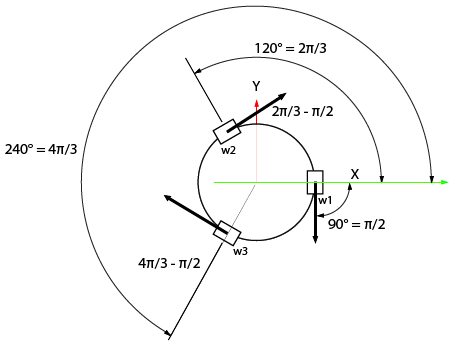
\includegraphics{figures/digram_model_dedution}
	\caption{Diagrama do robô}
\end{figure}

\begin{equation}
    \begin{split}
        \overrightarrow{V}_{l} = 
        \overrightarrow{V}_{w1}
        + \overrightarrow{V}_{w2}
        + \overrightarrow{V}_{w3}
    \end{split}
\end{equation}

\begin{equation}
    \begin{split}
        \overrightarrow{\omega} = 
        \frac{\vert\overrightarrow{V}_{w1}\vert}{L}
        + \frac{\vert\overrightarrow{V}_{w2}\vert}{L}
        + \frac{\vert\overrightarrow{V}_{w3}\vert}{L}
    \end{split}
\end{equation}


\begin{gather*}
        V_{l} \angle \theta =  
        V_{w1} \angle \left(-\frac{\pi}{2}\right) 
        + V_{w2} \angle \left(\frac{2\pi}{3}-\frac{\pi}{2}\right) 
        + V_{w3} \angle \left(\frac{4\pi}{3}-\frac{\pi}{2}\right) 
\end{gather*}

\begin{align*}
    V_{l} \cos{ \theta } + jV_{l} \sin{\theta} =  
    V_{w1} \cos{ \left(-\frac{\pi}{2}\right)} + jV_{w1} \sin{ \left(-\frac{\pi}{2}\right) } \\
    + V_{w2}  \cos{ \left(\frac{\pi}{6}\right) } + jV_{w2}  \sin{ \left(\frac{\pi}{6}\right) }  \\
    + V_{w3} \cos{ \left(\frac{5\pi}{6}\right) } + jV_{w2}  \sin{ \left(\frac{5\pi}{6}\right) } 
\end{align*}

\begin{equation*}
    \begin{split}
        \omega = 
        \frac{V_{w1}}{L}
        + \frac{V_{w2}}{L}
        + \frac{V_{w3}}{L}
    \end{split}
\end{equation*}


\begin{gather}
	\begin{bmatrix} V\cdot \cos{\theta} \\  V\cdot \sin{\theta} \\  \omega \end{bmatrix}
	=
	\begin{bmatrix}
		\cos{\left(-\frac{\pi}{2}\right)} & \cos{\left(\frac{\pi}{6}\right)} & \cos{\left(\frac{5\pi}{6}\right)} \\
		\sin{\left(-\frac{\pi}{2}\right)} & \sin{\left(\frac{\pi}{6}\right)} & \sin{\left(\frac{5\pi}{6}\right)} \\
		\frac{1}{L} & \frac{1}{L} & \frac{1}{L}
	\end{bmatrix}
	\cdot
	\begin{bmatrix} V_{w1} \\  V_{w2} \\  V_{w3} \end{bmatrix}
\end{gather}


Matriz da cinemática direta.

\begin{gather}
	\begin{bmatrix}
		\cos{\left(-\frac{\pi}{2}\right)} & \cos{\left(\frac{\pi}{6}\right)} & \cos{\left(\frac{5\pi}{6}\right)} \\
		\sin{\left(-\frac{\pi}{2}\right)} & \sin{\left(\frac{\pi}{6}\right)} & \sin{\left(\frac{5\pi}{6}\right)} \\
		\frac{1}{L} & \frac{1}{L} & \frac{1}{L}
	\end{bmatrix}
	=
	\begin{bmatrix}
		0 & \sqrt{3}/2 & -\sqrt{3}/2 \\
		1 & -1/2 & -1/2  \\
		1/L & 1/L & 1/L
	\end{bmatrix}
\end{gather}



Matriz inversa.


\begin{gather}
	\begin{bmatrix} V_{w1} \\  V_{w2} \\  V_{w3} \end{bmatrix}
	=
	\begin{bmatrix}
		0 & 2/3 & L/3 \\
		-1/\sqrt{3} & -1/3 & L/3\\
		1/\sqrt{3} & -1/3 & L/3
	\end{bmatrix}
	\cdot
	\begin{bmatrix} V\cdot \cos{\theta} \\  V\cdot \sin{\theta} \\  \omega \end{bmatrix}
\end{gather}



\section{Omni Wheel}

$V_{w}$ é velocidade linear da roda, $r$ raio da roda, $\omega_{w} $ é a velocidade angular da roda.


\[V_{w1} = \omega_{w1}\cdot r \] 


	
	

\chapter{Componentes}

\section{a}



\begin{quadro}[htb]
\caption{\label{lista de componentes}Componentes}
 \begin{tabular}{|c|c|c|c|}
	\hline
	\textbf{Componente} & \textbf{Quant} \\ \hline
	Motor DC 6V,  210 RPM, encoder integrado & 3  \\ \hline
	Driver Motor Ponte H L298n  & 3  \\ \hline
	Raspberry Pi 4    & 1   \\ \hline
	STM32 F103C8T6 & 2     \\ \hline
	Bateria & 1     \\ \hline
\end{tabular}
\fonte{Autor.}
\end{quadro}


%https://www.filipeflop.com/produto/driver-motor-ponte-h-l298n/
%https://www.filipeflop.com/produto/motor-dc-6v-com-encoder/?attribute_pa_rpm=210-rpm#tab-description

	

\chapter{Resultados}

\section{a}



	% ----------------------------------------------------------
	% Finaliza a parte no bookmark do PDF
	% para que se inicie o bookmark na raiz
	% e adiciona espaço de parte no Sumário
	% ----------------------------------------------------------
	\phantompart


	% Conclusão
	\chapter{Conclusão}
% ---

\lipsum[1]


	

% ELEMENTOS PÓS-TEXTUAIS
\postextual

	% Referências bibliográficas
	%\bibliography{abntex2-modelo-references}
	\bibliography{bibliography/bibliografia.bib}
	%\printbibliography

	% Glossário
	%\glossary



	% Apêndices
	\begin{apendicesenv}

% Imprime uma página indicando o início dos apêndices
% \partapendices




\chapter{Transcrição da matriz de cinemática em um bloco de código C \label{matriz_cinematica_c}}

\lstset{language=C}
\begin{lstlisting}
#include <math.h>
#define RADIUS_ROBOT 100
// mm, raio medido do centro ate o centro geometrico de cada roda
#define DEFAULT_SPEED 400 // mm/second   velocidade linear do robo.
#define RADIUS_WHEEL 34.5 //mm Raio da roda
#define PI 3.141592653589

float speedLinearToRpm(float speedLinear){
    float rpm = 60*speedLinear/(2*PI*RADIUS_WHEEL);
    return rpm;
}

void TransformationMatrixRpm(
	volatile long *w1, volatile long *w2, volatile long *w3,
	float linSpdPer, // percentagem da velocidade linear
	float dirAngle, float angSpd
){
	float linSpd_x, linSpd_y;
	linSpd_x = linSpdPer * DEFAULT_SPEED * cos(dirAngle * (PI/180));
	linSpd_y = linSpdPer * DEFAULT_SPEED * sin(dirAngle * (PI/180));

	float a1[3] = {0, -2.0/3,  RADIUS_ROBOT/3};
	float a2[3] = {1/sqrt(3), 1.0/3, RADIUS_ROBOT/3};
	float a3[3] = {-1/sqrt(3), 1.0/3, RADIUS_ROBOT/3};

	float spdLin1, spdLin2, spdLin3;
	spdLin1 = (a1[0] * linSpd_y) + (a1[1] * linSpd_x) + (a1[2] * angSpd);
	spdLin2 = (a2[0] * linSpd_y) + (a2[1] * linSpd_x) + (a2[2] * angSpd);
	spdLin3 = (a3[0] * linSpd_y) + (a3[1] * linSpd_x) + (a3[2] * angSpd);
	
	*w1 = speedLinearToRpm(spdLin1);
	*w2 = speedLinearToRpm(spdLin2);
	*w3 = speedLinearToRpm(spdLin3);	
}
\end{lstlisting}


\chapter{Transcrição da conversão de RGB para HSV em um bloco de código C \label{anx_rgb_to_hsv}}

\lstset{language=C}
\begin{lstlisting}
#include <stdio.h>
float maxOfThree(float a, float b, float c) {
	if ((a >= b) && (a >= c)) return a;
	else if ((b >= a) && (b >= c)) return b;
	else return c;
}
float minOfThree(float a, float b, float c) {
	if ((a <= b) && (a <= c)) return a;
	else if ((b <= a) && (b <= c)) return b;
	else return c;
}
void rgbToDirAngAndMag(int r, int g, int b, float *h, float *s) {
	float r_norm = r / 255.0, g_norm = g / 255.0, b_norm = b / 255.0;
	float cmax = maxOfThree(r_norm, g_norm, b_norm);
	float cmin = minOfThree(r_norm, g_norm, b_norm);
	float diff = cmax - cmin;
	if (cmax == cmin) {
		*h = 0;
	} else if (cmax == r_norm) {
		*h = fmod((60 * ((g_norm - b_norm) / diff) + 360), 360);
	} else if (cmax == g_norm) {
		*h = fmod((60 * ((b_norm - r_norm) / diff) + 120), 360);
	} else if (cmax == b_norm) {
		*h = fmod((60 * ((r_norm - g_norm) / diff) + 240), 360);
	}
	if (cmax == 0) {*s = 0;} else {*s = (diff / cmax) * 100;}
	*h = 360 - *h;
}
void main() {
	int r = 255, g = 0, b = 255; float h, s;
	rgbToDirAngAndMag(r, g, b, &h, &s);
	printf("Direction (Hue): %.2f\n", h); // res = 60
	printf("Magnitude (Saturation): %.2f\n", s); // res = 100
}
	
\end{lstlisting}
% 
\chapter{apendice 2}

\lipsum[1]


\end{apendicesenv}

	% Anexos
	\begin{anexosenv}

% Imprime uma página indicando o início dos anexos
\partanexos

\chapter{Cálculo modelo de 3 rodas}

\begin{figure}[h]
	\centering
	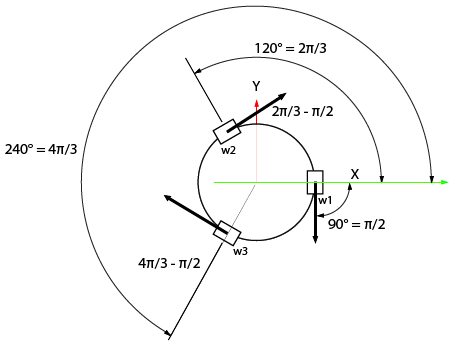
\includegraphics{figures/digram_model_dedution}
	\caption{diagrama do modelo - dedução da matriz}
	\label{lof}
\end{figure}

\begin{equation}
    \begin{split}
        \overrightarrow{V}_{l} = 
        \overrightarrow{V}_{w1}
        + \overrightarrow{V}_{w2}
        + \overrightarrow{V}_{w3}
    \end{split}
\end{equation}

\begin{equation}
    \begin{split}
        \overrightarrow{\omega} = 
        \frac{\vert\overrightarrow{V}_{w1}\vert}{L}
        + \frac{\vert\overrightarrow{V}_{w2}\vert}{L}
        + \frac{\vert\overrightarrow{V}_{w3}\vert}{L}
    \end{split}
\end{equation}


\begin{gather*}
        \dot{V}_{l} \angle \theta =  
        \dot{V}_{w1} \angle \left(-\frac{\pi}{2}\right) 
        + \dot{V}_{w2} \angle \left(\frac{2\pi}{3}-\frac{\pi}{2}\right) 
        + \dot{V}_{w3} \angle \left(\frac{4\pi}{3}-\frac{\pi}{2}\right) 
\end{gather*}

\begin{align*}
    \dot{V}_{l} \cos{ \theta } + j\dot{V}_{l} \sin{\theta} =  
    \dot{V}_{w1} \cos{ \left(-\frac{\pi}{2}\right)} + j\dot{V}_{w1} \sin{ \left(-\frac{\pi}{2}\right) } \\
    + \dot{V}_{w2}  \cos{ \left(\frac{\pi}{6}\right) } + j\dot{V}_{w2}  \sin{ \left(\frac{\pi}{6}\right) }  \\
    + \dot{V}_{w3} \cos{ \left(\frac{5\pi}{6}\right) } + j\dot{V}_{w2}  \sin{ \left(\frac{5\pi}{6}\right) } 
\end{align*}

\begin{equation*}
    \begin{split}
        \dot{\omega} = 
        \frac{\dot{V}_{w1}}{L}
        + \frac{\dot{V}_{w2}}{L}
        + \frac{\dot{V}_{w3}}{L}
    \end{split}
\end{equation*}


\begin{gather}
	\begin{bmatrix} \dot{V}\cdot \cos{\theta} \\  \dot{V}\cdot \sin{\theta} \\  \dot{\omega} \end{bmatrix}
	=
	\begin{bmatrix}
		\cos{\left(-\frac{\pi}{2}\right)} & \cos{\left(\frac{\pi}{6}\right)} & \cos{\left(\frac{5\pi}{6}\right)} \\
		\sin{\left(-\frac{\pi}{2}\right)} & \sin{\left(\frac{\pi}{6}\right)} & \sin{\left(\frac{5\pi}{6}\right)} \\
		\frac{1}{L} & \frac{1}{L} & \frac{1}{L}
	\end{bmatrix}
	\cdot
	\begin{bmatrix} \dot{V}_{w1} \\  \dot{V}_{w2} \\  \dot{V}_{w3} \end{bmatrix}
\end{gather}



\begin{gather}
	\begin{bmatrix} \dot{V}_{w1} \\  \dot{V}_{w2} \\  \dot{V}_{w3} \end{bmatrix}
	=
	\begin{bmatrix}
		0 & 2/3 & L/3 \\
		-1/\sqrt{3} & -1/3 & L/3\\
		1/\sqrt{3} & -1/3 & L/3
	\end{bmatrix}
	\cdot
	\begin{bmatrix} \dot{V}\cdot \cos{\theta} \\  \dot{V}\cdot \sin{\theta} \\  \dot{\omega} \end{bmatrix}
\end{gather}

\chapter{Outro Anexo}


\lipsum[32]



\end{anexosenv}



%---------------------------------------------------------------------
% INDICE REMISSIVO
%---------------------------------------------------------------------
\phantompart
\printindex


\end{document}

